\documentclass[a4paper,17pt]{extarticle}
\usepackage{geometry}
\usepackage[utf8]{inputenc}
\usepackage[table,xcdraw]{xcolor}
\usepackage{mathtools}
\usepackage{amsthm}
\usepackage{amsmath}
\usepackage{amsfonts}
\usepackage{amssymb}
\usepackage{centernot}
\usepackage{marvosym}
\usepackage{enumitem}
\usepackage{hyperref}
\setcounter{tocdepth}{1}
\theoremstyle{definition}
\newtheorem{definition}{Definition}
\let\marvosymLightning\Lightning
\renewcommand{\skip}{\par\null\par}
\newcommand{\T}{\mathcal T}
\renewcommand{\O}{\mathcal{O}}
\renewcommand{\Lightning}{\scalebox{1.5}{\marvosymLightning}}
\renewcommand{\L}{\mathcal{L}}
\renewcommand{\leq}{\leqslant}
\renewcommand{\geq}{\geqslant}
\newtheorem{theorem}{Theorem}
\newtheorem{corollary}{Corollary}[theorem]
\newtheorem*{remark}{Remark}
\renewcommand\qedsymbol{QED}
\newcommand{\R}{\mathbb{R}}
\newcommand{\N}{\mathbb{N}}
\newcommand{\Z}{\mathbb{Z}}
\newcommand{\divby}{%
  \mathrel{\text{\vbox{\baselineskip.65ex\lineskiplimit0pt\hbox{.}\hbox{.}\hbox{.}}}}%
  }
\newcommand{\notdivby}{\centernot\divby}
\title{\scalebox{1.5}{Math 553 Final Exam}}
\author{\scalebox{1.5}{Theo Koss}}
\date{May 2022}
\begin{document}
\maketitle
\begin{enumerate}
\item Let $v$ and $w$ be vector fields along a parameterized curve $\alpha: I\to S$ on an oriented regular surface $S$, with unit normal vector $N:S\to\R^3$. Show that $\frac{d}{dt}\langle v,w\rangle=\langle \frac{Dv}{dt},w\rangle+\langle v,\frac{Dw}{dt}\rangle$.\begin{proof}$$\frac{d}{dt}\langle v,w\rangle=\langle v',w\rangle+\langle v,w'\rangle$$ Then, since $v'$ and $w'$ are both tangents to $S$, we can break them into components: $$v'=\frac{Dv}{dt}+v_n$$ and likewise for $w'$. Where $\frac{Dv}{dt}$ represents the tangential component of $v'$ and $v_n$ represents the normal component. Then, by definition, $v_n$ is orthogonal to $w$ and therefore $\langle v_n,w\rangle=0$. Similarly $\langle v,w_n\rangle=0$. Now differentiating:\begin{align*}
    \frac{d}{dt}\langle v,w\rangle&=\langle v',w\rangle+\langle v,w'\rangle\\
    &=\langle \frac{Dv}{dt}+v_n,w\rangle+\langle v,\frac{Dw}{dt}+w_n\rangle\\
    &=\langle \frac{Dv}{dt},w\rangle+\langle v_n,w\rangle+\langle v,\frac{Dw}{dt}\rangle+\langle v,w_n\rangle\\
    &=\langle \frac{Dv}{dt},w\rangle+\langle v,\frac{Dw}{dt}\rangle
\end{align*}
As required.
\end{proof}
\item Suppose that $S$ has a coordinate patch $(U,\phi)$. Recall that the curve $(u(t),v(t))$ in $U$ determines a geodesic on $S$ provided the geodesic equations are satisfied. i.e. $$u''+(u')^2\Gamma_{11}^1+2u'v'\Gamma_{12}^1+(v')^2\Gamma_{22}^1=0$$ $$v''+(u')^2\Gamma_{11}^2+2u'v'\Gamma_{12}^2+(v')^2\Gamma_{22}^2=0$$ Now suppose as well that $(U,\phi)$ is isothermal, in that the coefficients of the first fundamental form satisfy $E=G=\lambda$ and $F=0$. Show that the geodesic equations become: $$2\lambda u''+(u')^2\lambda_u+2u'v'\lambda_v-(v')^2\lambda_u=0$$ $$2\lambda v''+(u')^2\lambda_v+2u'v'\lambda_u-(v')^2\lambda_v=0$$ \begin{proof} According to Do Carmo pp. 239, working out the Christoffel symbols given $E=G=\lambda$ and $F=0$: $$\Gamma_{11}^1=\frac{1}{2}\frac{\lambda_u}{\lambda},\ \Gamma_{11}^2=-\frac{1}{2}\frac{\lambda_v}{\lambda}$$ 
$$\Gamma_{12}^1=\frac{1}{2}\frac{\lambda_v}{\lambda}\ \Gamma_{12}^2=\frac{1}{2}\frac{\lambda_u}{\lambda}$$
$$\Gamma_{22}^1=-\frac{1}{2}\frac{\lambda_u}{\lambda},\ \gamma_{22}^2=\frac{1}{2}\frac{\lambda_v}{\lambda}$$
Therefore the first geodesic equation becomes $$u''+(u')^2\frac{1}{2}\frac{\lambda_u}{\lambda}+2u'v'\frac{1}{2}\frac{\lambda_v}{\lambda}+(v')^2(-\frac{1}{2}\frac{\lambda_u}{\lambda})=0$$ Then, multiplying everything by $2\lambda$ to get rid of the denominator: $$\implies 2\lambda u''+(u')^2\lambda_u+2u'v'\lambda_v-(v')^2\lambda_u=0$$ As required. The second equation follows similarly.
\end{proof}
\item Consider the surface $\mathbb{H}=\{(x,y)\in\R^2:y>0\}$, endowed with first fundamental form $\emph{I}_{(x,y)}=\frac{dx^2+dy^2}{y^2}$.\begin{enumerate}[label=(\roman*)]
    \item Compute curvature of $\mathbb{H}$ using $K=\frac{1}{2\lambda}\Delta(\log{\lambda})$.\skip We know $E=G=\lambda=\frac{1}{y^2}$. So $\frac{1}{2\lambda}=\frac{y^2}{2}$.\newline The Laplacian is then:\begin{align*}
        \Delta(\log\lambda)&=\left(\frac{\partial^2\log\lambda}{\partial x^2}\right)+\left(\frac{\partial^2\log\lambda}{\partial y^2}\right)\\
        &=\left(\frac{\partial^2\log\lambda}{\partial y^2}\right)\\
        &=\frac{\partial}{\partial y}\left(-\frac{2}{y}\right)\\
        &=\frac{2}{y^2}
    \end{align*}
    So $K=\frac{1}{2\lambda}\Delta(\log{\lambda})=\frac{y^2}{2}\cdot\frac{2}{y^2}=1$.
    \item Let $\gamma:\left(-\frac{\pi}{2},\frac{\pi}{2}\right)\to\mathbb{H}$ be given by $$\gamma(t)=(x_0+r\tanh{t},r\text{sech }t)$$ where $x_0\in\R$. Draw a picture of $\gamma(t)$, and show that $\gamma$ is PBAL, in that $\emph{I}_{\gamma(t)}(\gamma'(t))=1$.\skip Picture (assuming $x_0=0$ and $r=1$. It is moved left or right depending on $x_0$ and scaled by $r$.)\newline\begin{center}
        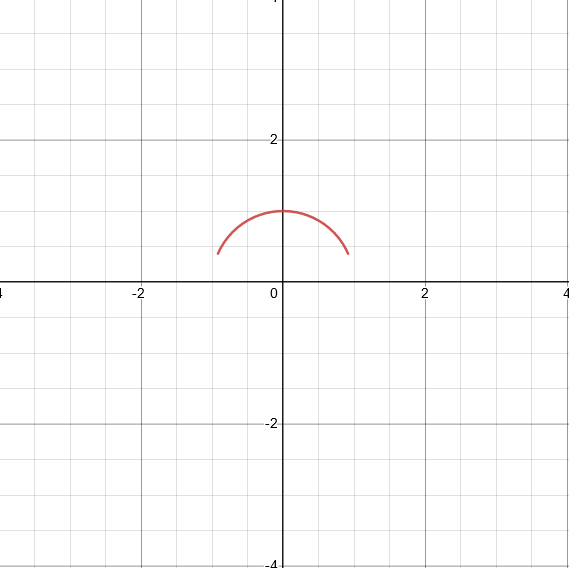
\includegraphics{parametric.PNG}
    \end{center}\skip $$E=r^2\text{sech}^4t$$ $$F=-r^2\tanh t\text{sech}^3t$$ $$G=r^2\tanh^2t\text{sech}^2t$$ $$L=\int_{-\frac{\pi}{2}}^{\frac{\pi}{2}}\sqrt{r^2\text{sech}^4t-r^2\tanh t\text{sech}^3t+r^2\tanh^2t\text{sech}^2t}dt$$ (This integral gave me an answer $\neq1$. Usually the curve is like $X(u,v)=...$ but it's different here so I'm a bit confused. I tried a couple ways but none of them worked out.)
    \item Use problem 2 to show the curve is geodesic.
    \item Does $\mathbb{H}$ have any other geodesics? Explain.
\end{enumerate}
\item Compute the Euler characteristic of a torus of revolution $T$, and explain why you can conclude that the integral of the Gaussian curvature over $T$ is equal to $0$.\begin{proof}By Do Carmo pp. 276, the torus is homeomorphic to a sphere with one handle, and from a result on that page, $$g=\frac{2-\chi(S)}{2}$$ Where $g$ denotes the number of handles on a surface. Plugging in 1 for $g$ it is easy to see that $\chi(S)=0$. Since Euler characteristic is a topological invariant, showing that $\chi(S)=0$ for $S\simeq T$ directly implies $\chi(T)=0$. Then, by the Gauss-Bonnet theorem, $$\iint_TKdA=2\pi\chi(T)$$ And since $\chi(T)=0$, we may conclude that $K=0$.
\end{proof} (Side note, this proof kind of feels like cheating because the result was in the text. I was trying to find a triangulation of the torus of revolution to show this more concretely but I couldn't find one.)
\item Let $\alpha:I\to\R^2$ be a simple, closed, regular curve, PBAL, in the plane, and let $\kappa:I\to\R$ be the (signed) curvature of $\alpha$. Use Gauss-Bonnet to show that $$\int_{\alpha}\kappa(s)ds=2\pi$$\begin{proof}Using the isometry $\R^2\to\R^3$ sending $(x,y)\to(x,y,0)$, consider the surface in 3 space given by $M=(x,y,0)$. This is isometric to $\alpha=(x,y)$. Now consider the Gauss-Bonnet theorem, using notation from eqn. 3 of \href{https://mathworld.wolfram.com/Gauss-BonnetFormula.html}{https://mathworld.wolfram.com/Gauss-BonnetFormula.html}: $$\iint_MKdA=2\pi\chi(M)-\sum\varphi_i-\int_{\partial M}\kappa_gds$$ Working through this notation:\begin{itemize}
    \item Our surface $M$ is defined by $M:=(x,y,0)$ which is homeomorphic to a disk, and therefore has Euler characteristic $\chi(M)=1$ and $K=0$.
    \item There is no ``jump angle'' $\varphi_i$ of $\alpha$ since $\alpha$ never intersects itself (it is simple), therefore the sum works out to be 0.
    \item $\partial M$ is the boundary of $M$, which is clearly $\alpha$. Then the geodesic curvature $\kappa_g$ is simply the curvature of $\alpha$. 
\end{itemize} Thus, the Gauss-Bonnet theorem simplifies to:\begin{align*}
    \int_{\partial M}\kappa_gds&=2\pi\\ \implies \int_{\alpha}\kappa(s)ds&=2\pi
\end{align*} As required.
\end{proof}
\end{enumerate}
\end{document}